\documentclass[class=article, crop=false]{standalone}
\usepackage[utf8]{inputenc}


\usepackage{amsfonts}
\usepackage{amsmath}
\usepackage[english]{babel}
\usepackage{booktabs}
\usepackage{caption}
\usepackage{graphicx}
\usepackage{import}
\usepackage{multicol}
\usepackage{multirow}
\usepackage[subpreambles=false]{standalone}
\usepackage{subcaption}
\usepackage{tikz}
\usepackage{float}
\usepackage{placeins}
\usepackage{stfloats}

\usepackage[linesnumbered,ruled,vlined]{algorithm2e}
\newcommand\commentfont[1]{\footnotesize\ttfamily\textcolor{blue}{#1}}
\SetCommentSty{commentfont}

\usepackage[backend=biber]{biblatex}
\addbibresource{references.bib}

\usepackage{geometry}
\geometry{
   a4paper,
   left=20mm, right=20mm,
   top=20mm, bottom=25mm
}
 
\usepackage{hyperref}
\hypersetup{
  colorlinks=true,
  linkcolor=blue,
  citecolor=black,
}

\usepackage{pgfplots}
\pgfplotsset{compat=1.3}
 
 
\setlength{\tabcolsep}{2pt} % Default value: 6pt
\renewcommand{\arraystretch}{1} % Default value: 1


\begin{document}
\twocolumn

\section{Experimental Setup}\label{sec:exp_setup}


Multiple experiments are performed to assess the models for facial landmark detection. The experiments involve testing which input is the most effective (point cloud or mesh input), evaluating the effectiveness of the refinement model different configurations, and assessing which input features (XYZ or HKS) are more suitable for the problem. Finally, the data augmentation technique horizontal flipping and color features are added to the experiments. The exact model configurations can be found in Table \ref{tab:configuration}.

We train the refinement model in two different configurations: The first has lower jittering ($j=3$mm) and a radius of the sphere of $r=2.5$cm. For the second network, we increase jittering to $j=6$mm and slightly increase the sphere radius to $r=3$cm to ensure that the true landmark is still within that radius.  

During training, the models are evaluated on a validation set. For each experiment, the model with the best accuracy is taken. The final evaluation in the next section is performed on a separate test set to ensure a reasonable estimate of a generalization error.
%TODO EARLY STOPPING
\begin{table*}[t]
\captionof{table}{\textbf{Model configuration.} Models are trained on an Nvidia Titan V. *Diffusion is truncated to an Eigenbasis of $k = 128$ for spectral acceleration.}

\centering
\begin{tabular}{l||c|c|c}\toprule
                & Initial Network XYZ & Initial Network HKS                                                                                               & Refinement Networks \\ \hline
$N$ Blocks         & 4                   & 8                                                                                                                 & 4                   \\
Block width $D$    & 256                 & 356                                                                                                               & 128                 \\
$F$ Input features & XYZ ( + RGB)        & HKS  & XYZ                 \\
Dropout         & 0.1                 & 0.1                                                                                                               & 0.1                 \\
Epochs          & 200                 & 550                                                                                                               & 200                 \\
Initial LR      & 1e-3                & 1e-3                                                                                                              & 1e-3                \\
LR decay factor & 0.5 per 80          & 0.5 per 200                                                                                                       & 0.5 per 80          \\
Optimizer       & Adam                & Adam                                                                                                              & Adam                \\
Size of eigenbasis k*      & 128                 & 128                                                                                                               & 128                 \\
Batch size      & 1                   & 1                                                                                                                 & 1                   \\
                &                     &                                                                                                                   &                  
\end{tabular}
\label{tab:configuration}
\end{table*}

\section{Results and Analysis}
\label{sec:results}
During training, the error metric used is the mean squared error between the actual and the predicted activation. While this is a valuable and differentiable metric for training the point-wise regression model, we are ultimately interested in the point landmarks. As described, the point landmarks are extracted by taking the point per channel with the maximum activation. Then, the results can be easily interpreted by calculating the difference between the actual and predicted landmarks. Because coordinates are given in millimeters, the difference is equivalent to the euclidean distance between the actual and the predicted landmark coordinate in millimeters. We compute the mean per landmark and the total mean for presenting results. Figure \ref{fig:pred_gt_pt} shows the visualization of an example with a relatively poor mean error of 4.40mm. The green dots are the actual, manually annotated landmarks and the red dots are the predicted landmarks.



The first experiments are performed on meshes and point clouds as input to compare the performance (see Table \ref{table:pcl_vs_mesh}). When using meshes, additionally to the vertices, also the face information is used by DiffusionNet to compute the operators. For the gradient computation, the 1-ring-neighbors are used instead of nearest neighbors for point clouds. Oddly, we observe a lower performance on meshes than point cloud input even though Sharp et al.\ generally observe superior results on meshes. The performance drop could be due to a faulty implementation but is not investigated further. Therefore, the remaining experiments are performed on the point cloud format. The training and evaluation are performed on the original noisy Headspace labels.
\begin{figure}[!htb]
\centering
  % \hspace*{-0.08\linewidth}
   
 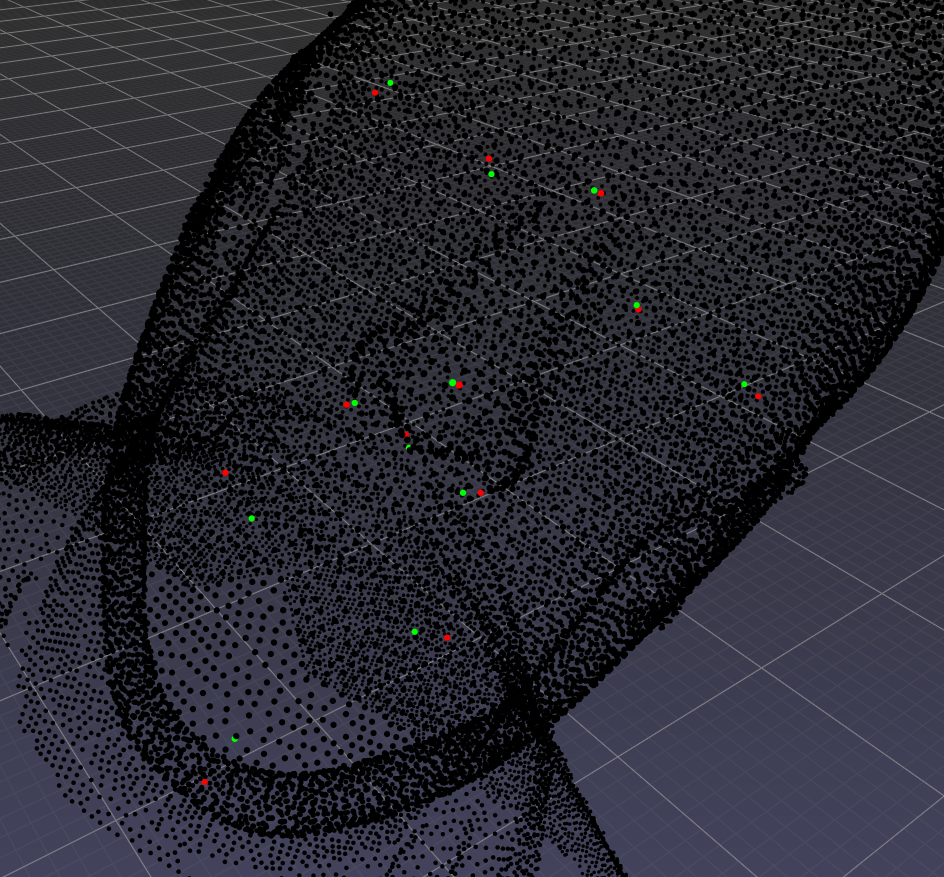
\includegraphics[width=\linewidth]{thesis/results/import/imgs/pred_gt_pt.png}
  %\vspace*{-0.06\linewidth}
 \captionof{figure}{
    \textbf{Result example.}
    \small Initial network predictions (red) against ground truth (green). The ground truth is a manual annotation of a Headspace sample. Sample mean error: 4.40mm. Landmark errors: \mbox{pg = 12.8mm}, \mbox{n = 1.3mm}, \mbox{prn = 1.1mm}, \mbox{ac-r = 1.8mm}, \mbox{sn = 3.4mm}, \mbox{ac-l = 3.3mm}, \mbox{ex-r = 3.8mm}, \mbox{en-r = 3.7mm}, \mbox{en-l = 0.9mm}, \mbox{ex-l = 4.0mm}, \mbox{ch-r = 10.2mm}, \mbox{ch-l = 6.4mm}.
  }
  \label{fig:pred_gt_pt}
\end{figure}
%\import{}{import/pred_gt_pt.tex}
\begin{table*}[!htbp]
\captionof{table}{\textbf{Point cloud versus mesh input.} The initial networks are trained on 1200 Headspace samples with the Headspace labels and XYZ features. Evaluating on Headspace labels instead of manual labels unsurprisingly yields better results because the network presented more similar targets during training and evaluation. In the experiments, training on meshes instead of point clouds leads to higher errors, which is why the remaining experiments are performed on the point cloud format.}
\label{table:pcl_vs_mesh}
\begin{tabularx}{\textwidth}{l|c|c}
\toprule
 & \multicolumn{2}{c}{Mean error in mm} \\\cmidrule(lr){2-3}
Landmark               & \hspace{0.3cm} Initial network (Point cloud) \hspace{0.3cm}  &  \hspace{0.3cm} Initial Network (Mesh) \hspace{0.3cm}      
\\
\midrule
Pogonion               & 4.08       & 7.44                                                                        \\
Nasion                 & 2.00       & 2.06  \\ %\pm
Pronasale              & 2.96       & 2.10 \\
Subnasale              & 2.81       & 2.97 \\
Exocanthion (right)    & 2.71       & 2.55 \\
Endocanthion (right)   & 2.51       & 2.40 \\
Endocanthion (left)    & 2.30       & 2.27 \\
Exocanthion (left)     & 3.07       & 2.28\\
Cheilion (right)       & 2.71       & 3.43 \\
Cheilion (left)        & 3.12       & 3.41 \\
\bottomrule
total & \textbf{2.825} & \textbf{3.120} 
\end{tabularx}
\end{table*}

The second round of experiments (see Table \ref{table:ref_hks}) are performed to assess the refinement network and see if an improvement to the predictions of the initial network can be observed. The refinement network indeed manages to improve upon the initial network's accuracy by over 0.6mm. 

Note that the training has been performed on the noisy Headspace labels, whereas the models were evaluated on the more accurate manual annotations, which explains why a drop of accuracy from 2.825mm to 3.731 mm can be observed. This gives reason to suspect that the ``noise" in the Headspace labels follows a pattern that the previous model learns.

As a part of this experimental setup, we also test a model trained on the rotation-invariant HKS features. The model performs significantly worse with a mean error of 5.386mm. The model especially fails to detect the Pogonion well, with a mean error of 13.9mm. Table \ref{table:ref_hks_max} reveals that in some cases, the prediction entirely fails with a maximum error of 11.0cm. This experiment is performed without alar curvature landmarks, thus the missing values in the table. This model, however, was not trained to its full potential because at 550 epochs, the training was cancelled due to long training times. As shown in the model configuration in Table \ref{tab:configuration}, a significantly more complex model is chosen with double the diffusion blocks and a higher block width. Still, likely, the model has not fully converged yet, and further training is necessary to judge its full potential. Another reason for the drop in performance might be the arising bilateral landmark issue, at least for the affected landmarks with a bilateral counterpart. 








%\newcolumntype{L}{>{\raggedright\arraybackslash}X}
\begin{table*}[!htbp]
\captionof{table}{\textbf{Refinement network assessment and HKS features.} The initial networks are trained on Headspace point clouds (110 manually labelled + 1100 Headspace labels) with XYZ and HKS features. The refinement network is trained on 110 manually labelled samples with XYZ features. All networks are evaluated on 30 manually labelled Headspace samples. The refinement network improves upon the initial network. The initial network trained on HKS clearly performs worse on pose normalized images. Maximum errors are listed in Appendix \ref{sec:app_results}, Table \ref{table:ref_hks_max}.
    }
\label{table:ref_hks}
\begin{tabularx}{\textwidth}{l|c|c|c}
\toprule
 & \multicolumn{3}{c}{Mean error $\pm$ std in mm} \\\cmidrule(lr){2-4}
Landmark               & \hspace{0.3cm}Initial Network (XYZ) \hspace{0.3cm}  & \hspace{0.3cm} Refinement Network (1) \hspace{0.3cm} & \hspace{0.3cm} Initial Network (HKS) \hspace{0.3cm}     
\\
\midrule
Pogonion               & 7.70 $\pm$ 3.44 & 4.78 $\pm$ 2.32 & 13.90 $\pm$ 18.26\\
Nasion                 & 2.76 $\pm$ 1.14 & 1.86 $\pm$ 0.62 & 3.31 $\pm$ 1.54\\
Pronasale              & 2.44 $\pm$ 1.16 & 1.86 $\pm$ 1.12 & 3.31 $\pm$ 1.65\\
Alar curvature (right) & 2.54 $\pm$ 1.41 & 2.08 $\pm$ 1.30 & -\\
Subnasale              & 2.87 $\pm$ 1.37 & 2.47 $\pm$ 1.23 & 3.28 $\pm$ 1.80\\
Alar curvature (left)  & 3.03 $\pm$ 1.35 & 2.66 $\pm$ 2.13 & - \\
Exocanthion (right)    & 5.13 $\pm$ 2.04 & 5.01 $\pm$ 2.22 & 5.38 $\pm$ 2.50\\
Endocanthion (right)   & 3.34 $\pm$ 1.56 & 2.38 $\pm$ 1.44 & 4.25 $\pm$ 1.97\\
Endocanthion (left)    & 2.35 $\pm$ 1.63 & 2.63 $\pm$ 2.13 & 4.08 $\pm$ 1.73\\
Exocanthion (left)     & 4.55 $\pm$ 2.25 & 4.04 $\pm$ 2.28 & 5.72 $\pm$ 2.82\\
Cheilion (right)       & 4.80 $\pm$ 2.18 & 4.18 $\pm$ 2.56 & 5.71 $\pm$ 7.62\\
Cheilion (left)        & 3.22 $\pm$ 2.14 & 2.96 $\pm$ 2.11 & 4.73 $\pm$ 3.44\\
\bottomrule
total & \textbf{3.731 $\pm$ 2.43} & \textbf{3.089 $\pm$ 2.18} & \textbf{5.386 $\pm$ 7.22}
\end{tabularx}
\end{table*}

For the refinement model, taking three samples of random translation of the center point proves effective as a slight increase of mean accuracy from 3.164 to 3.089 was observed.

In the last round of experiments, the models are trained solely on the more accurate manual annotations. For the initial network, the data is augmented by horizontal flipping. Additionally, the input dimension $F$ increases from 3 to 6 as RGB features are added to the input. With this setup, the initial network achieves a lower mean error of 2.779mm (see Table \ref{table:horizflip_rgb}). Refinement model (1) with lower jittering improves the accuracy to 2.548mm. Refinement model (2) with higher jittering achieves the best results with a mean error of 2.217mm.

\begin{table*}[!htbp]
\captionof{table}{\textbf{Horizontal flipping and color features.} Both, the initial and refinement network are trained on 277 manually labelled Headspace point clouds. As before, the evaluation is done on 30 manually labelled Headspace samples. The initial network is trained on XYZ features enrichened with RGB information and horizontal flipping is performed during training to double the training set. These measures and more training samples with accurate labels achieve the highest accuracy in our experiments. The refined network slightly improves upon that accuracy. Maximum errors are listed in Appendix \ref{sec:app_results}, Table \ref{table:horizflip_rgb_max}.}
\label{table:horizflip_rgb}
\begin{tabularx}{\textwidth}{l|c|c|c}
\toprule
 & \multicolumn{3}{c}{Mean error $\pm$ std in mm} \\\cmidrule(lr){2-4}
Landmark               & \hspace{0.5cm}Initial network\hspace{0.5cm} &  \hspace{0.5cm}Refinement network (1)   \hspace{0.5cm} & \hspace{0.5cm} Refinement network (2)  \hspace{0.5cm}
\\
\midrule
Pogonion               & 3.33 $\pm$ 2.00 & 3.23 $\pm$ 1.99 & 2.68 $\pm$ 1.73 \\
Nasion                 & 2.24 $\pm$ 1.32 & 2.47 $\pm$ 1.91 & 2.50 $\pm$ 2.00\\  
Pronasale              & 2.35 $\pm$ 1.27 & 1.50 $\pm$ 0.84 & 1.33 $\pm$ 0.84\\
Alar curvature (right) & 1.99 $\pm$ 1.28 & 2.48 $\pm$ 1.87 & 2.29 $\pm$ 1.98\\
Subnasale              & 1.86 $\pm$ 0.84 & 1.53 $\pm$ 0.97 & 1.29 $\pm$ 0.89\\
Alar curvature (left)  & 2.05 $\pm$ 1.20 & 1.74 $\pm$ 0.98 & 1.70 $\pm$ 1.03\\   
Exocanthion (right)    & 2.44 $\pm$ 1.76 & 2.28 $\pm$ 1.46 & 2.05 $\pm$ 1.30\\ 
Endocanthion (right)   & 2.54 $\pm$ 1.91 & 2.66 $\pm$ 1.77 & 1.92 $\pm$ 1.31\\ 
Endocanthion (left)    & 3.23 $\pm$ 1.74 & 3.26 $\pm$ 2.16 & 2.39 $\pm$ 1.70\\
Exocanthion (left)     & 2.69 $\pm$ 1.32 & 3.34 $\pm$ 2.12 & 2.95 $\pm$ 2.06\\
Cheilion (right)       & 3.61 $\pm$ 3.01 & 2.76 $\pm$ 1.72 & 2.70 $\pm$ 1.82\\
Cheilion (left)        & 5.00 $\pm$ 3.85 & 3.32 $\pm$ 2.36 & 2.83 $\pm$ 1.58\\

\bottomrule
total & \textbf{2.779 $\pm$ 2.16} & \textbf{2.548 $\pm$ 1.87} & \textbf{2.217 $\pm$ 1.67}
\end{tabularx}
\end{table*}


Remarkably, we use the original landmark coordinates as the ground truth for calculating the results, not the recalculated point-wise targets that the networks are trained on. As Section \ref{sec_data_preparation} describes, the targets are recalculated by picking the closest point to the original landmark. Consequently, even with a point-wise prediction an error of zero millimeters is practically impossible because the true landmark point is not sampled as an input point. The reason for that is twofold: Firstly, the landmarking in 3DMedX saves arbitrary coordinates and not pointers to vertices. Secondly, the initial network uses the downsampled mesh. Here, the targets are recalculated for the low-resolution point cloud. Only for the high-resolution point clouds with Headspace labels, the original landmarks are equivalent to the targets used as input to the networks, allowing predictions of zero millimeters to be recorded (but these experiments are not listed in the results in this work). Experiments show that the difference between the ground truth used for the final evaluation of the initial network and the low-resolution network targets cause an overestimation of the error of around 0.2mm. Thus, if the initial network would predict every landmark perfectly, the final evaluation would still yield an error of around 0.2mm due to the low-resolution approximation. Nonetheless, we consciously decide to evaluate the network in that manner to allow a fair comparison between the initial network and the refinement network. The initial network's performance is thus slightly better than the results might convey.

% which landmarks are easier to detect than others?


% applying on meshes, applying on high resolution test samples...

% tell about effect of weighted mse

% Qualitative results for UMC controls

% hyperparameters

\subsection{Radboudumc data}
% XYZ rotate points vs HKS
Despite the poor results of HKS compared to XYZ features on the Headspace data, we find that models trained on HKS features are more widely applicable to 3D meshes ``in the wild". Such meshes are typically not consistently oriented. The initial network trained on XYZ features fails to learn meaningful features in such cases. Augmentation by random rotation helps prepare the network for inconsistently oriented faces, but the performance is still inferior. These findings indicate that the space of possible rotation in 3D is too large to be simulated with data augmentation. Therefore, we resort to training the networks on HKS features, making the network more difficult to train, but showing acceptable detection performance on the Radboudumc data. No quantitative results are available because the data does not come with landmark annotations. Figure \ref{fig:2} shows an example prediction of the initial network trained on HKS features.\documentclass[crop=false]{standalone}

\usepackage[subpreambles=false]{standalone}
\usepackage{import}
\usepackage{graphicx}
\usepackage{subcaption}
\usepackage{tikz}

\begin{document}

\begin{figure}
  \centering
  % \hspace*{-0.08\linewidth}
     \begin{subfigure}[b]{0.2278\textwidth}
  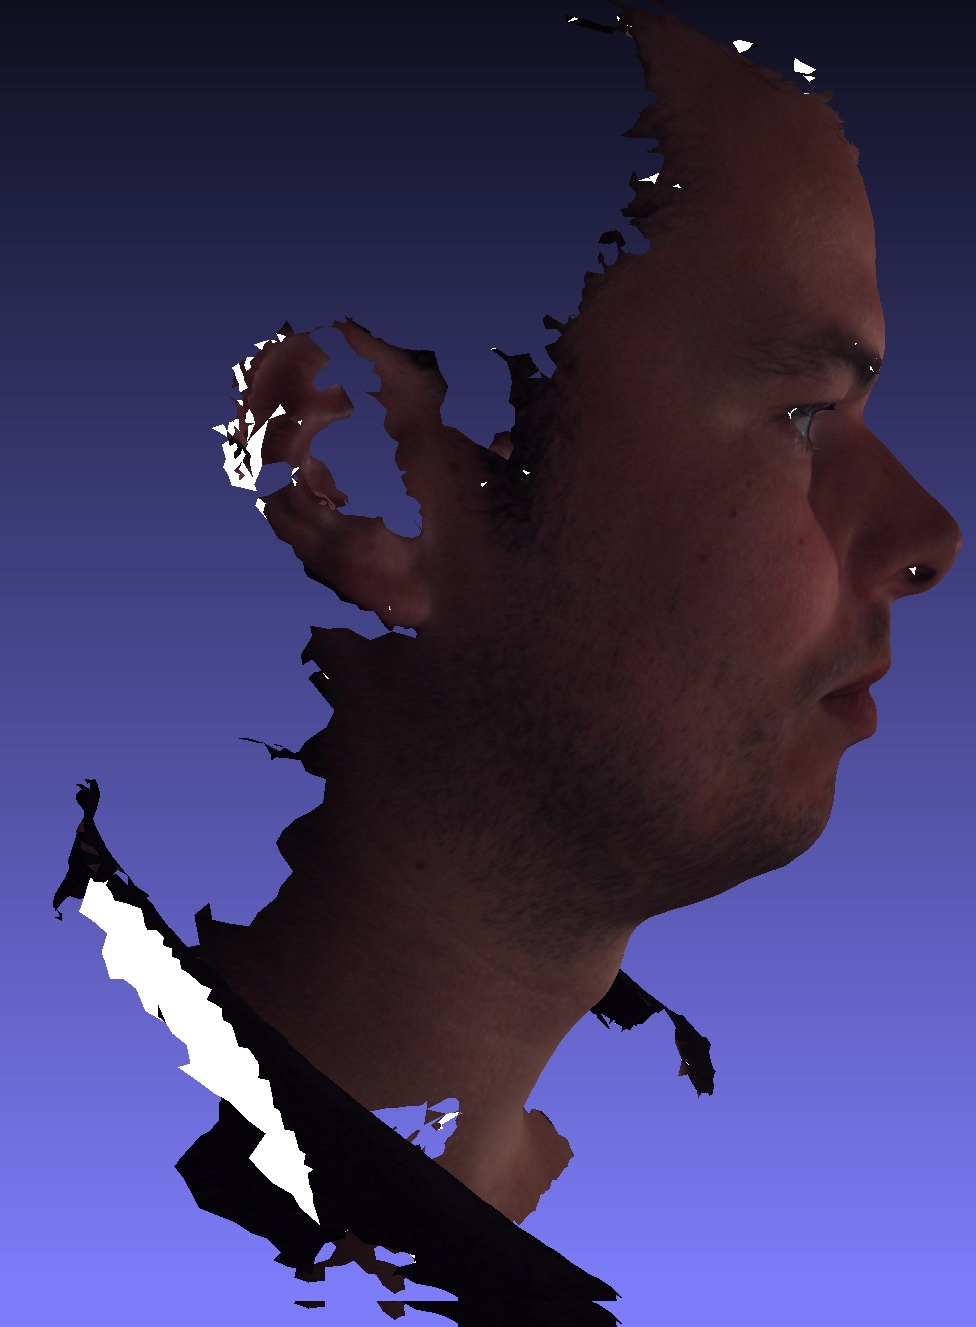
\includegraphics[width=\textwidth]{thesis/results/import/imgs/Untitled6.jpg}
  \caption{}
  \label{fig:1}
  \end{subfigure}
  \begin{subfigure}[b]{0.2282\textwidth}
   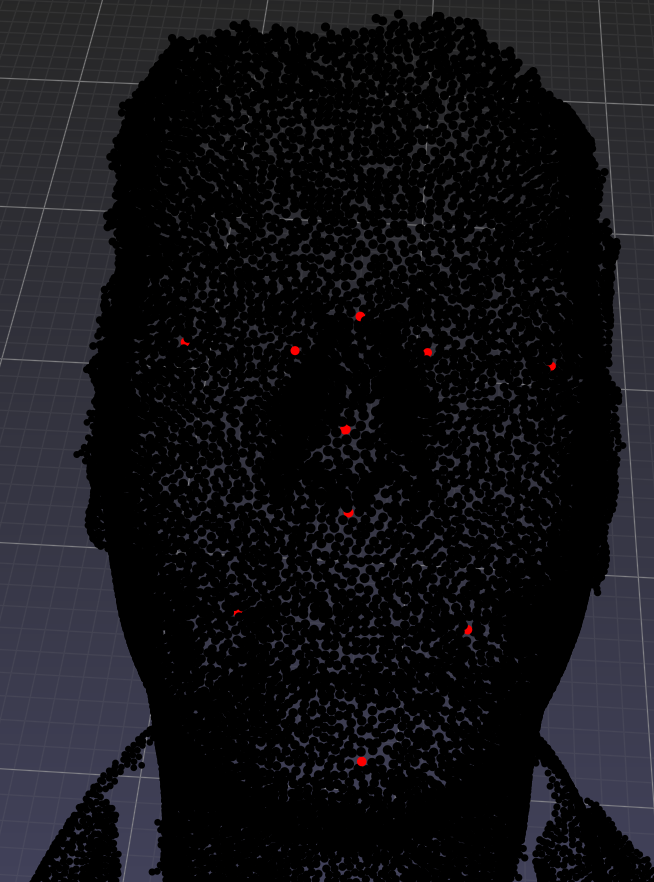
\includegraphics[width=\textwidth]{thesis/results/import/imgs/3.png}
   \caption{}
   \label{fig:2}
   \end{subfigure}
  %\vspace*{-0.06\linewidth}
  \caption{\textbf{Radboudumc prediction example.} \small (a) Side profile of the original mesh. The photo was captured by two cameras, capturing only the face. The head is oriented differently to the pose normalized samples in the training set. The lower mesh quality is also visible in the texture, demonstrated as white spots for faulty textures. (b) Frontal profile of the same subject showing predictions. At first glance, the predictions look seemingly accurate. Quantitative results on Headspace annotations indicate however, that the model trained on HKS is more inaccurate with a mean error over 5mm. 
    
   }
   \label{fig:pred_umc_datax} 
  
\end{figure}

\end{document}  

\end{document}
